% !TeX spellcheck = en_US
% !TeX encoding = UTF-8
% !TeX root = ../document.tex

\newcommand{\sigmatrue}{\ensuremath{\sigma_\text{true}}\xspace}

\chapter{Statistical Evaluation}
\section{Coverage Analysis}
\label{sec:coverage}

In this chapter, we will investigate to what extend the test statistic \TS introduced in \fref{sec:test_statistic} can be directly interpreted as $p$-value, as intended: $p = \TS$. For that purpose, we will refer to the definition and requirements of a $p$-value and test whether \TS fulfills those requirements.
Additionally, we will repeat the analysis with \TSprime, using the log-normal prior (as suggested in \fref{sec:test_statistic}) instead of the Gaussian term in \TS and compare the results.

A $p$-value is an indicator for the significance of a deviation, where a smaller $p$-value corresponds to a higher significance. The $p$-value of a result is compared to a significance threshold $\alpha$, which is fixed before the statistical analysis. If the observed $p$-value is smaller than $\alpha$, the null hypothesis is rejected\cite{Cowan:StatisticsSearchesLHC}. In our case, rejection of the null hypothesis corresponds to falsification of the \acl{SM} and thus the discovery of new physics. 

Both values are constructed in a way that the null hypothesis is (incorrectly) rejected by chance with a probability of $\alpha$:
\begin{align}
	\Pr( H_0\:\text{rejected} | H_0 ) &= \alpha \\
    \label{eq:coverage_inequality}
    \Rightarrow \Pr( p < \alpha | H_0 ) &= \alpha
\end{align}
This equation is tested during the \emph{coverage analysis}.

In the case of \TS, a deviation from this equality is expected. One reason for that is the truncation of the normal distribution. 
Usually, the probability of including the true value in a certain interval around the expected value is the same as including an expected value in an interval with the same width around the true value:
\begin{align}
    &\Pr(\Nmc - x \cdot \sigma \leq \Ntrue < \Nmc + x \cdot \sigma) \\
    = &\Pr(\Ntrue - x \cdot \sigma \leq \Nmc < \Ntrue + x \cdot \sigma)
\end{align}
This property holds for all $x$ if the probability density is a (non-truncated) normal distribution.
Truncation however breaks this property. 
The effect becomes more visible as the truncated probability increases and therefore should be most dominant in areas of very large uncertainty.

\subsection{Procedure}
To test \fref{eq:coverage_inequality}, we construct pseudo experiments based on the null hypothesis $H_0$ and calculate the corresponding $p$-value, in this case \TS or \TSprime. After generating and examining sufficiently many pseudo experiments, we can determine the rate of significant findings and compare them to the claimed significance threshold:
\begin{equation}
	p_\text{true} = \frac{\text{number of pseudo-experiments where $p < \alpha$}}{n_\text{toys}} = \Pr(p < \alpha | H_0)
    \label{eq:coverage}
\end{equation}

The pseudo experiments are based on \acs{MUSiC}'s null hypothesis: 
We assume that there is a constant probability that events end up in a particular region, and thus a constant true mean value \Ntrue. 
We also assume that this true mean value is only known up to an expected event yield, \Nmc.
The way that \Nmc is derived from \Ntrue differs between \TS and \TSprime: For \TS, \Nmc is drawn from a normal probability density, \TSprime  will use a log-normal distribution instead.

Additionally, the physics process of performing a counting experiment has to be simulated: Here it is assumed that the event yield is caused by independent statistical processes with a fixed probability, thus the observed event yield follows a Poisson distribution around \Ntrue.

The way that the assumed uncertainty enters the pseudo experiment also differs between \TS and \TSprime: For \TS, the absolute uncertainty is kept constant: $\sigmamc = \sigmatrue$. For \TSprime, we recalculate the uncertainty after drawing \Nmc in order to keep the relative uncertainty constant: $\sigmamc = \frac{\Nmc}{\Ntrue} \sigmatrue$.
This has been discussed by \cite{Schmitz:ModelUnspecificSearch}, a more rigorous discussion can be found in \fref{app:coverage_uncertainty}.

In the implementation, each pseudo-experiment begins with drawing \Nmc from the probability density around \Ntrue. At the same time, \Ndata is drawn from a (discrete) Poisson distribution with a mean of \Ntrue. From these two values, as well as the uncertainty \sigmamc, \TS (or \TSprime) is calculated.

This process is repeated for $n_\text{toys}$ pseudo-experiments. An estimation for the true $p$ value is afterwards calculated using \fref{eq:coverage}, which yields the left hand side of \fref{eq:coverage_inequality}.

In order to state the so called "coverage value" for the tuple (\Ntrue, \sigmatrue), both sides of  \fref{eq:coverage_inequality} are translated to $Z$-scores (see \fref{app:z_score}), resulting in $Z_\text{true} = Z(p_\text{true})$ representing the observed and $Z_\text{claim} = Z(\alpha)$ representing the claimed rate ob significant results.
The coverage is finally reported as
\begin{equation}
    \label{eq:coverage_value}
	\Delta Z \defeq Z_\text{true} - Z_\text{claim}.
\end{equation}
%or alternatively as 
%\begin{equation}
%    \text{coverage}' = \log_{10} %\left(\frac{p_\text{true}}{p_\text{claim}}\right)
%\end{equation}

\subsection{Possible Outcomes}
Three different result cases can arise, depending on the coverage value in \fref{eq:coverage_value}:
\begin{enumerate}
	\item $\Delta Z = 0 \Leftrightarrow \Pr( H_0 \text{ rejected} | H_0 ) = \alpha$: This is the ideal case. It indicates the $p$-value performs according to its definition.
	\item $\Delta Z < 0 \Leftrightarrow \Pr( H_0 \text{ rejected} | H_0 ) > \alpha$: The background hypothesis is rejected more often than with a probability of $\alpha$. This case is called "undercoverage" and corresponds to "liberal" behavior. The $p$-value overestimates the significance of deviations.
	\item $\Delta Z > 0 \Leftrightarrow \Pr( H_0 \text{ rejected} | H_0 ) < \alpha$: The background hypothesis is not rejected in some cases where it should have been rejected. This effect is called "overcoverage" and corresponds to "conservative" behavior where the $p$-value underestimates the significance of deviations.
\end{enumerate}	

\subsection{Results}
Since the MUSiC $p$-value is required to cover a large range of possible \Ntrue and relative uncertainty $\sigmatrue / \Ntrue$ values, the coverage is evaluated on a two dimensional grid in this parameter space.
The computed results for \TS can be found in \fref{fig:coverage_normal}, for \TSprime in \fref{fig:coverage_lognormal}. 

\begin{figure}
    \centering
    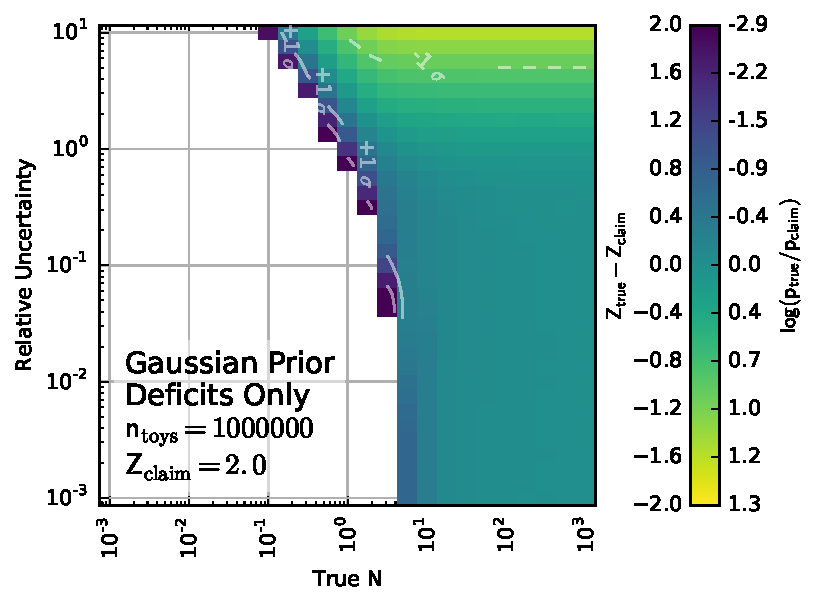
\includegraphics[width=0.9\textwidth]{coverage/coverage_deficit_normal_log}
    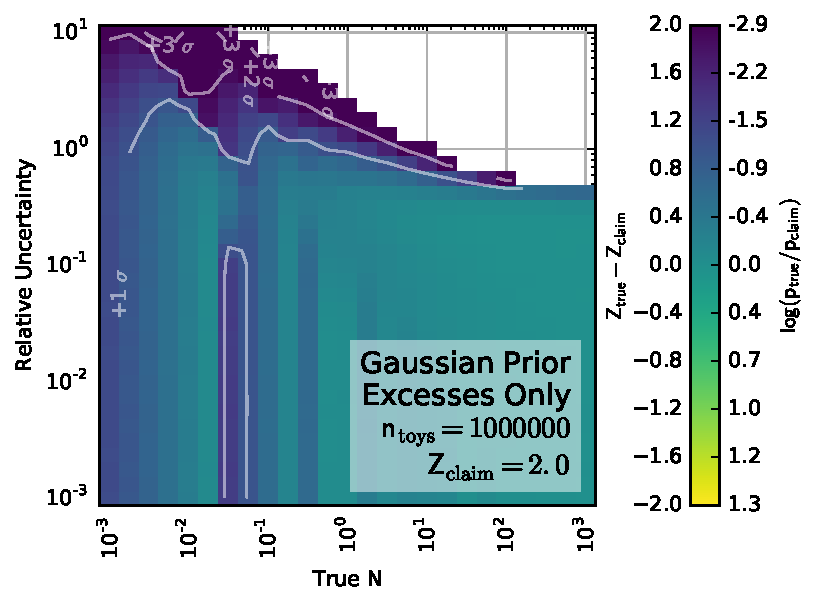
\includegraphics[width=0.9\textwidth]{coverage/coverage_excess_normal_log}
    \caption{Results of the coverage analysis for \TS, using the Gaussian prior. The figure on top shows that coverage for deficits, the bottom figure indicates coverage behavior for excesses. Within the blank areas, the coverage value could not be determined since no significant result could be observed.}
    \label{fig:coverage_normal}
\end{figure}

\begin{figure}
    \centering
    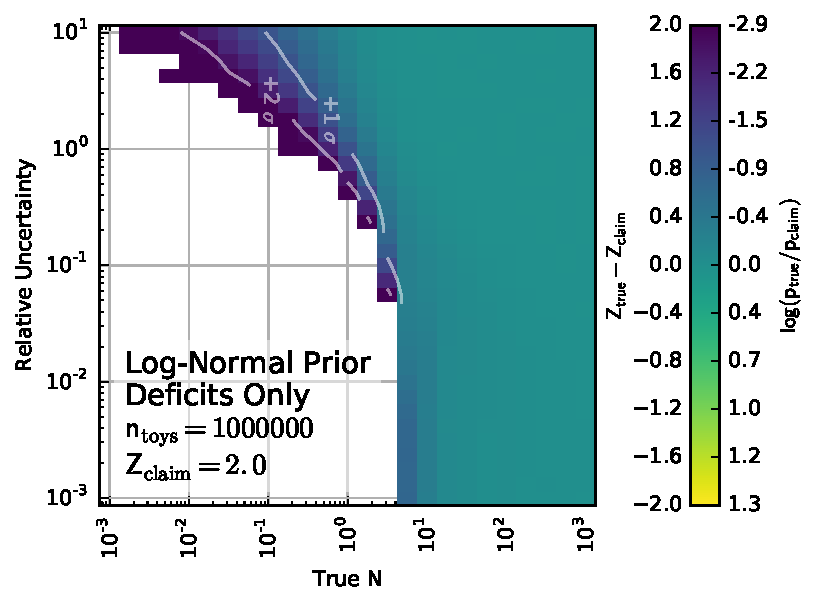
\includegraphics[width=0.9\textwidth]{coverage/coverage_deficit_lognormal_log}
    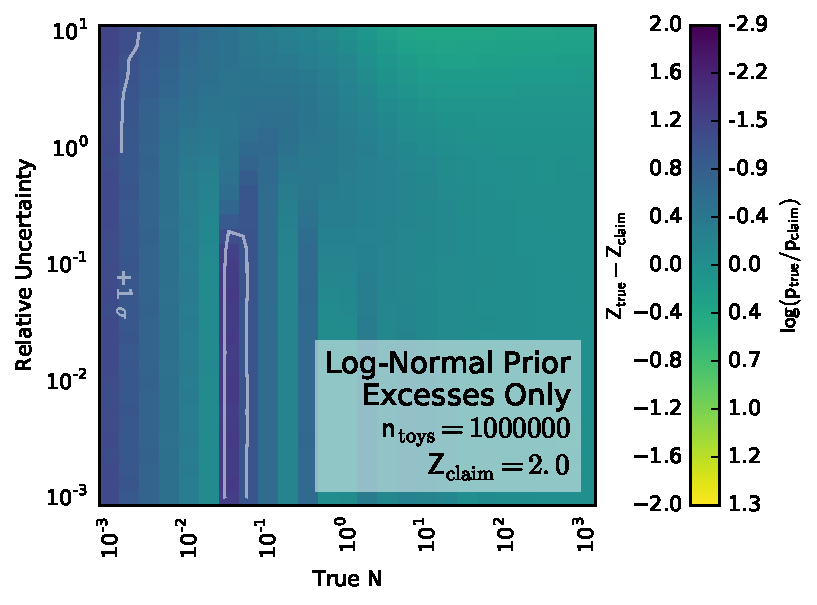
\includegraphics[width=0.9\textwidth]{coverage/coverage_excess_lognormal_log}
    \caption{Results of the coverage analysis for \TSprime, using the log-normal prior. The figure on top shows that coverage for deficits, the bottom figure indicates coverage behavior for excesses.}
    \label{fig:coverage_lognormal}
\end{figure}

Areas tinted with dark blue color were determined to be overcovered (conservative behavior), while the bright yellow shows areas of undercoverage. Within the blank areas, the coverage value could not be determined since no significant result could be observed. This is expected, especially for deficits below $\Ntrue = \num{1}$, because at $\Nmc < \num{1}$, the only possible deficit is $\Ndata = \num{0}$, which is not significant purely by the Poisson contribution in \TS ($p \geq e^{-1} = \num{0.37}$ with $\sigmamc \rightarrow \num{0}$).

Further illustrations in non-logarithmic view can be found in \fref{app:coverage_additional_results}.

\subsubsection{Results for \TS}
For the Gaussian prior in \TS, one can see almost ideal coverage for $\Ntrue > \num{1}$ and $\sigmamc/\Ntrue < \SI{50}{\percent}$. This is compatible with the results from earlier studies\cite{Schmitz:ModelUnspecificSearch}, which have been reproduced partially in \fref{app:coverage_schmitz}.

As expected, the coverage equality breaks down at large uncertainties: In the deficit case undercoverage becomes visible, while the excess case shows overcoverage. 
For several regions, the \TS-value is too conservative, leading to the effect that not a single significant round can be obtained during the coverage study. In these regions, the coverage value cannot be computed and therefore the area is displayed blank.

%Agressiv mit def reluncert->inf weil exp(-lambda) term.
% excess, uncert -> inf => p->1

% deficit, uncert -> inf => p->0 siehe Script truncated_normal
% C -> linear in \sigma, integral -> 1 ==> p = ratio -> 0

\subsubsection{Results for \TSprime}
The log-normal prior shows much better coverage values across the probed range. There are areas of slight overcoverage, but especially in the excess case the overcoverage does not exceed $\num{1} \sigma$.

\subsection{Discussion}
We have conducted a coverage analysis of the local test statistic \TS with a Gaussian and a log-normal prior. As expected, the Gaussian prior shows deficiencies especially at high values of relative uncertainty. 
One apparent solution would be to correct the \TS-value with a parametrized correction factor to reestablish perfect coverage. In practice, it is not obvious how to parametrize the coverage difference in all three ($\Ndata, \Nmc, \sigmamc$) dimensions. Therefore, this approach is not further pursued in this thesis.

In comparison, the log-normal prior performs well over the entire tested range, with a coverage of $\abs{\Delta Z} \leq 1$. 
Therefore, if the goal of the local test statistic is to correspond to the definition of a $p$-value, the log-normal prior is to prefer over the Gaussian prior. 

\section{Log-Normal $p$-Value}
\label{sec:lognormal_pvalue}

As observed in the previous section, using the truncated Gaussian distribution as prior within the $p$-value has limited validity at high relative uncertainties.
At the same time, we have observed that using a log-normal prior improves test coverage in the problematic regions.

In addition, a log-normal prior is more suited for modeling our uncertainties: Analogously to the normal distribution, which is generated from a sum of independent random variables, the log-normal distribution results from the multiplication of independent random variables (see \fref{app:lognormal_derivation}). The latter corresponds to our situation, as most uncertainties on the event yield originate from shifting the event yield by a multiplicative factor.
Also note that in the limit of $\Nmc \rightarrow \infty$ and $\sigmamc \rightarrow 0$, the log-normal distribution recovers the shape of a normal distribution, which explains similar coverage properties in that region.

Changing the prior in the test statistic also implies a new null-hypothesis, namely that all uncertainties are distributed in a log-normal fashion. Therefore, the pseudo-experiment generation, which is based on the null-hypothesis, must also be adapted. Instead of choosing a new pseudo-mean value using a sum of uncertainties multiplied by a normally distributed bias (see \fref{eq:pseudo_experiment_mean}), one now has to use a product of relative uncertainties:
\begin{equation}
    \Ntrue' = \Nmc \cdot \prod_i \left(1 + \frac{\sigma_i}{\Nmc}\right)^{x_i}
\end{equation}

However, this approach also comes with its disadvantages: When combining multiple bins into a region, previously we added individual bin contents. Assuming normally distributed bin contents, this approach is valid because the sum of two normally distributed random variables is also normally distributed. Yet, this principle does not apply to log-normal distributions. The sum of log-normally distributed random variables is not log-normally distributed.

In the following, we want to discuss some solutions to this challenge, some of which have been discussed in previous works on the log-normal prior\cite{Schmitz:ModelUnspecificSearch}.

\begin{itemize}
    \item Use Gaussian error propagation in any case: While this solution may approximately hold for two bins with the same number of events and relative uncertainty, it breaks down with more unequal numbers as the combined distribution differs significantly from the distribution obtained by summation of two (or more) random numbers drawn separately.
    \item Use an approximation: The challenge of approximating a sum of log-normally distributed random variables is of interest for various applications and has therefore been thoroughly researched. The oldest, most popular approach is the Fenton-Wilkinson approximation which is obtained by matching mean and variance of the sum to a log-normal distribution. Unfortunately, this approach breaks down when combining more than two bins \cite{Pirinen:Statisticalpowersum}.
    Other possible alternatives are the Schwartz-Yeh approximation \cite{Schwartz:DistributionFunctionMoments}, which matches the first two moments of the logarithms with additional weight functions, and a recent procedure by Mehta et. al.\cite{Mehta:ApproximatingSumCorrelated} which uses a Gauss-Hermite approximation and poses the most accurate solution. The downside of the latter approaches is that they are computationally expensive, involving the calculation of integrals.
    Since a region can consist out of up to $\sim \num{100}$ bins, the number of regions per event class can reach up to $\sim \num{10000}$. Thus using a computationally cheap algorithm is absolutely necessary. Because of the high number of parameters (two for each bin) using a \ac{LUT} is also not feasible.
    \item Combine bins to regions first, generate pseudo-experiments on the complete regions instead of bins: This approach completely ignores the direct correlation between overlapping regions, and therefore does not represent our null-hypothesis.
    \item Generate pseudo-experiments from a normal distribution, evaluate the \TS-value with the log-normal prior: This approach has been pursued in an earlier signal study\cite{Schmitz:ModelUnspecificSearch}. As this signal study was performed before the start of data taking at \ac{CMS}, uncertainties were underestimated. With larger uncertainties, this procedure is no longer feasible. The problem can be illustrated using an example from the turn-on region of the distribution. The uncertainty in these areas mostly originates from distribution shifts and therefore can be very large. Using a Gaussian prior, the scenario $\Nmc = \num{1000} \pm \num{2000}, \Ndata = \num{0}$ yields a \TS-value of \num{0.00025}, while a log-normal prior would assign \num{2.5e-8}. This tension of $\num{1.9}\sigma$ causes very significant pseudo-experiments in these regions of large uncertainties and large event numbers.
\end{itemize}

Although the problem of combining bins is the only problem arising from a log-normal prior, it is so grave that the log-normal prior will not be used for the signal study in this thesis. Instead, an alternative solution to the overcoverage of the normal \TS-value will be presented in the next section.

\section{Region Veto Against Overcoverage}
\label{sec:overcoverage_veto}

In \fref{sec:region_veto}, several rules have been introduced to prevent inference for regions with incomplete simulation.
In this section, we will add another rule, which however does not intend to limit the search space because of invalid input for the test statistic, but to avoid shortcomings of the Gaussian test statistic itself.

In \fref{sec:coverage}, it was shown that the test statistic \TS with the Gaussian prior has severe overcoverage for regions of high relative systematic uncertainty. We will now introduce a simple rule excluding these problematic regions from our search.
In the bottom plot of \fref{fig:coverage_lognormal}, we can see that the contour line $\text{coverage} = +2\sigma$ follows a straight path in double logarithmic presentation. This line can be approximately parametrized with 
\begin{equation}
   \frac{\sigmamc}{\Ntrue} =  \num{1.2} \cdot \Ntrue^{-0.2}
\end{equation}
Regions with a larger systematic uncertainty (above the line) should be excluded from the search due to insufficient coverage of the test statistic.

As \Nmc is our best estimator for \Ntrue, we will also replace \Ntrue with \Nmc. Additionally, in order not to unnecessarily veto regions with large \Ntrue, and not to diverge at $\Nmc \rightarrow 0$, this value is restricted to the range between \num{0.5} and \num{5.0}:
\begin{equation}
    \frac{\sigmamc}{\Nmc} = \max(\num{0.5}, \min(\num{1.2} \cdot \Nmc^{-0.2}, \num{5.0}))
\end{equation}

The excluded area is illustrated in \fref{fig:coverage_veto}.

\begin{figure}
    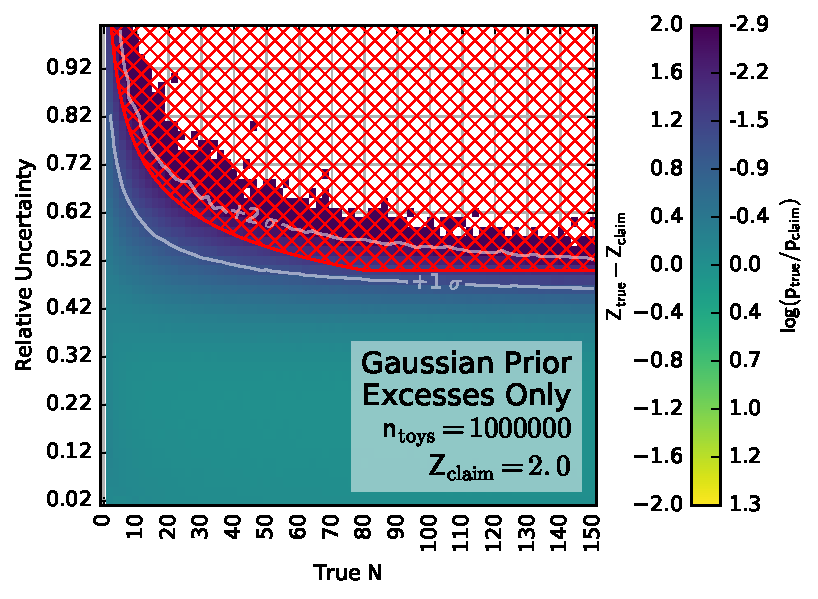
\includegraphics[width=\textwidth]{coverage/coverage_excess_normal_lin_thresh}
    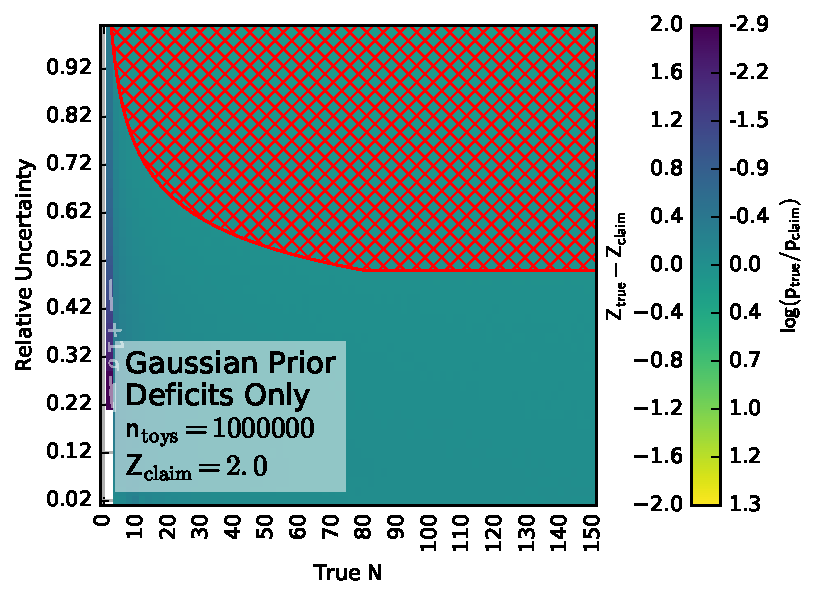
\includegraphics[width=\textwidth]{coverage/coverage_deficit_normal_lin_thresh}
    \caption{Illustration of the regions vetoed due to insufficient coverage (areas with red hatching pattern).}
    \label{fig:coverage_veto}
\end{figure}

\section{A Global $p$-Value}
\label{sec:global_pvalue}

The \ptilde distribution provides the ability to notice an increase of not very significant deviations in many classes by inspecting the central part of the distribution. However, this manual method is only qualitative. We will now introduce a possible extension to the analysis which provides a quantitative method of combining all \ptilde-values of a search in one kinematic variable for all classes.

This allows us not only to draw conclusions about the presence of new physics in our observed data set, but also to quantify \ac{MUSiC}'s sensitivity for simulations of known benchmark models. Furthermore, an automated analysis can be used as a regression test to decide whether future modifications to the analysis improve its sensitivity.

As input, the algorithm takes the look-elsewhere-corrected \ptilde values of all classes. In the case of \ac{MC} simulation, either for \ac{SM} or signal studies, such a set of \ptilde values can be provided for each pseudo experiment round, for observed data we only obtain one list (one value for each class).

The algorithm for the \ac{SM} distribution performs as follows: For each pseudo experiment round, the distribution of \ptilde values (of all classes) is compared to a reference distribution using a statistical test. The reference distribution is the distribution of all \ptilde values of \ac{SM}-only pseudo-experiments, of all \nclasses event classes and \nrounds pseudo-experiment rounds, as presented in \fref{fig:phat_reference}. Note that the distribution features a spike at $\ptilde \approx 1$, which originates from the remaining discretization of \ptilde discussed in \fref{sec:min_yield}. 

\begin{figure}
    \centering
    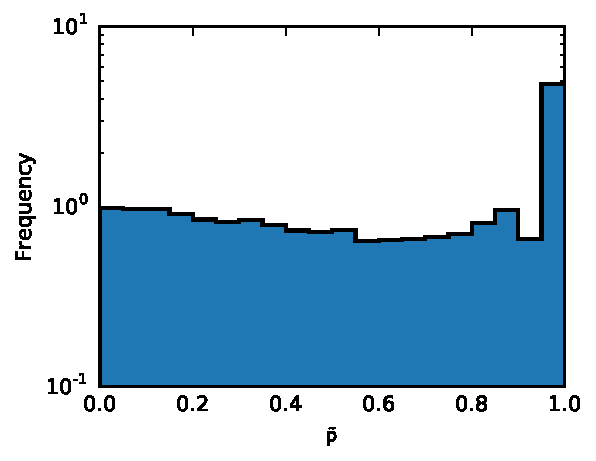
\includegraphics[width=0.6\textwidth]{reference_plot}
    \caption{Reference distribution $g(\ptilde)$, serving as input to the analysis. In this instance, the \sumpT distribution has been analyzed, shown are all \ptilde values of exclusive event classes.}
    \label{fig:phat_reference}
\end{figure}

The statistical test outputs a scalar result \TSphat for each of the \nrounds rounds, where a larger value indicates a larger deviation from the reference distribution. The set of \nrounds test statistic values is stored.
Given a single observed \ptilde distribution, one can analogously compute the test statistic \TSphatdata. The \phat value is then defined as
\begin{equation}
    \phat = \Pr(\TSphat > \TSphatdata | H_0),
\end{equation}
where $H_0$ indicates the null hypothesis given by the \acl{SM}.
For a decision whether or not the null hypothesis should be rejected, \phat has to be compared to a significance threshold $\alpha$. $\alpha$ is equivalent to the type-I error rate, the probability of incorrectly rejecting the null hypothesis if it were true\cite{Cowan:StatisticsSearchesLHC}:
\begin{equation}
    \Pr(\phat < \alpha | H_0) = \alpha
\end{equation}
Equivalently, a critical value \TSphatcrit of the test statistic can be defined, such that 
\begin{equation}
    \Pr(\TSphat > \TSphatcrit | H_0) = \alpha
\end{equation}

Similarly, the type-II error rate can be identified, which denotes the probability of incorrectly accepting $H_0$ if it is false\cite{Cowan:StatisticsSearchesLHC}:
\begin{equation}
    \Pr(\phat > \alpha | H_1) = \Pr(\TSphat < \TSphatcrit | H_1) = \beta
\end{equation}
The quantity $1 - \beta$ is called \emph{test power}\cite{Cowan:StatisticsSearchesLHC} and in our case indicates the probability of correctly rejecting the \ac{SM} if the dataset under investigation contains new physics. The test power of a test therefore directly describes the sensitivity towards a particular new physics scenario.

The test power can be calculated from simulations of new physics, such as the combined signal and background pseudo-experiments as described in \fref{sec:signal_study}. The test power does not only depend on the chosen test statistic and signal model, but also on $\alpha$. A larger value of $\alpha$ is less restrictive and will correctly accept the alternative hypothesis more often, at the cost of incorrectly rejecting the \ac{SM}.

The choice of $\alpha$ is subjective\cite{Cowan:StatisticalMethodsDiscovery}. Rather than following a strict convention, it is important to state which significance threshold has been used and, if the test statistic indicates that the null hypothesis should be discarded, to act accordingly. In the case of the \ac{MUSiC} analysis, finding a deviation from the \ac{SM} would certainly initiate a dedicated analysis at \ac{CMS}. Therefore, we can afford to set an aggressively high value of $\alpha = \SI{5}{\percent}$\footnote{For comparison, a discovery in particle physics is usually claimed at $\alpha \sim \num{e-7}$\cite{Cowan:StatisticsSearchesLHC}.}, and accepting the fact that in \SI{5}{\percent} of the cases, we would incorrectly reject the \ac{SM} and trigger a dedicated analysis.

So far, the choice of the test statistic \TSphat has not been specified. In the following, multiple options are discussed. The distribution of \ptilde values under investigation is denoted as $f(\ptilde)$, having $N_f = \nrounds$ values, the reference distribution is $g(\ptilde)$, with $N_g$ values. The cumulative distribution functions are $F(\ptilde)$ and $G(\ptilde)$ respectively. 

\begin{itemize}
    \item $\chi^2$-Test\cite{Cowan:Statisticaldataanalysis,Flannery:NumericalrecipesFORTRAN}: This test is used to compare two sets of values, binned into distributions. For each bin $i$, the difference between bin contents $g'_i$ for the reference and the sample bin content $f'_i$ is evaluated.
    \begin{equation}
        \TSphat = \frac{\chi^2}{\text{ndof}} = \frac{1}{\text{number of bins}} \sum_i^{\text{bins}} \frac{\left(\sqrt{N_g/N_f} \cdot f'_i - \sqrt{N_f/N_g} \cdot g'_i\right)^2}{N_f + N_g}
    \end{equation}
    
    A disadvantage of this method is that binning discards information. Additionally, the method works best for large number of event classes.
    
    \item Kolmogorov-Smirnov\cite{Flannery:NumericalrecipesFORTRAN,Darling:kolmogorovsmirnovcramer}: This test does not require binning. It compares the empirical cumulative distribution functions of reference and comparison, finding the maximal distance between $F$ and $G$.
    \begin{equation}
        \TSphat = \left(\sqrt{N_e} + \num{0.12} + \num{0.11}/\sqrt{N_e}\right) \cdot \sup_i \abs{F(\ptilde_i) - G(\ptilde_i)}
    \end{equation}
    where 
    \begin{equation}
        N_e = \frac{N_f \cdot N_g}{N_f + N_g}
    \end{equation}
    is an effective number of values.
    
    A disadvantage of this test statistic is that it is most sensitive to deviations in the center of the distribution. Additionally, only the largest difference is used for the result, instead of accumulating the difference.
    
%    \item Cramér-von-Mises\cite{Stephens:EDFstatisticsgoodness}: The Cramér-von-Mises test statistic consists of the integral over the quadratic difference between the reference and compared cumulative distribution functions:
%    \begin{equation}
%        \TSphat = \nrounds \int_{-\infty}^{\infty}\left(F(x) - G(x)\right)^2 w(x)\, \dd F(x) 
%    \end{equation}
%    where $w(x) = 1$. 
%    The discrete version of this test for comparing to a uniform distribution is:
%    \begin{equation}
%        \TSphat = \frac{1}{12 \nrounds} + \sum_{i=1}^\nrounds \left[\frac{2i-1}{2\nrounds} - F(\ptilde_i)\right]^2
%    \end{equation}
    
    \item Anderson-Darling\cite{Stephens:EDFstatisticsgoodness,Darling:kolmogorovsmirnovcramer,Flannery:NumericalrecipesFORTRAN}: This test belongs to the group of quadratic EDF\footnote{EDF = empirical distribution function} statistics. This group consists of test statistics that integrate over the quadratic difference between the reference and sample cumulative functions:
    \begin{equation}
        \TSphat = \nrounds \int_{-\infty}^{\infty}\left(F(x) - G(x)\right)^2 w(x)\, \dd F(x) 
    \end{equation}
    Here, the weighting term $w(x)$ can be used to focus on specific parts of the distribution. The simplest possible weight is $w(x) = 1$, which is used by the Cramér-von-Mises test statistic.
    The Anderson-Darling metric uses a more sophisticated weight $w(x) = \left[G(x)(1 - G(x))\right]^{-1}$ instead, giving more weight to both tails of the distribution.
    
    For this thesis, the discrete two-sample version is used, which is described in \cite{Scholz:KsampleAnderson}.
    
    \item Simple: \TSphat is the ratio of \ptilde values below a critical value, in this case \num{0.01}.
\end{itemize}

A thorough comparison of the afore-mentioned test statistics can be found in \cite{Stephens:EDFstatisticsgoodness}.

Alternatively, the reference distribution can be replaced by a uniform distribution. This also simplifies the formulas of most test statistics. Additionally, this variant has the advantage of enabling the analyst to identify whether the \ac{SM}-only distribution agrees with our assumptions. However, as we will see in \fref{chap:sensitivity_studies}, the comparison to a uniform distribution can only be done with a higher minimum yield threshold of e.g. $\Nmc \geq \num{1.0}$, which reduces the number of event classes with $\ptilde \approx 1$ and therefore brings each distribution closer to a uniform distribution.
